% begin module concavity-def
\begin{frame}
\frametitle{What Does $f''$ Say About $f$?}
$f$ and $g$ are both increasing functions on $(a,b)$ with the same end points, but they look different because they bend in different directions.
\begin{columns}[c]
\column{.5\textwidth}
\ \only<handout:0| -2>{%
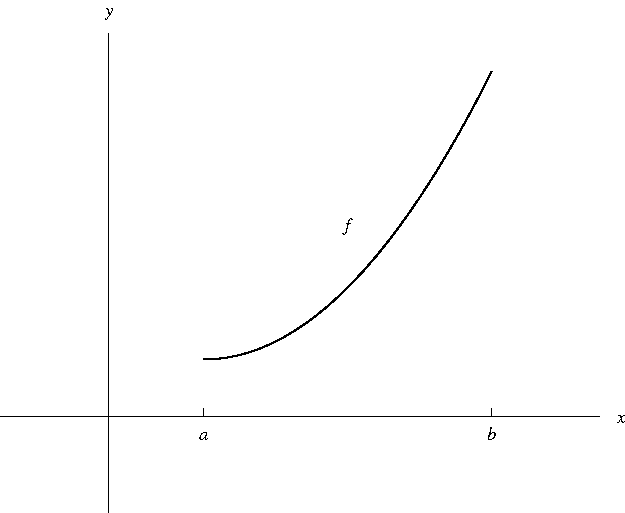
\includegraphics[height=3.5cm]{curve-sketching/pictures/04-03-concaveupa.pdf}%
}%
\only<handout:0| 3>{%
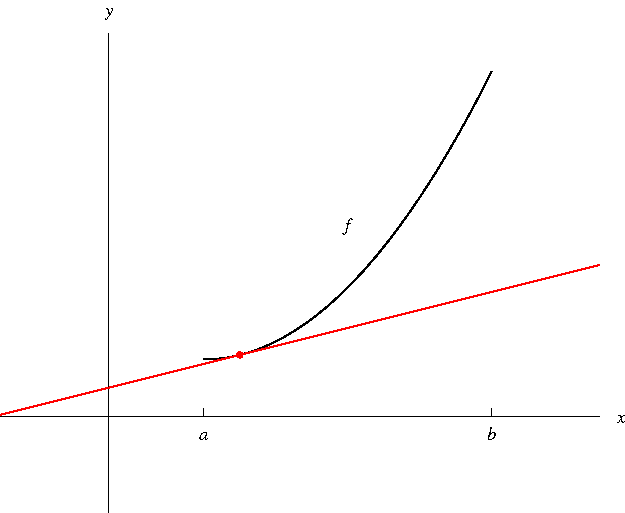
\includegraphics[height=3.5cm]{curve-sketching/pictures/04-03-concaveupb.pdf}%
}%
\only<handout:0| 4>{%
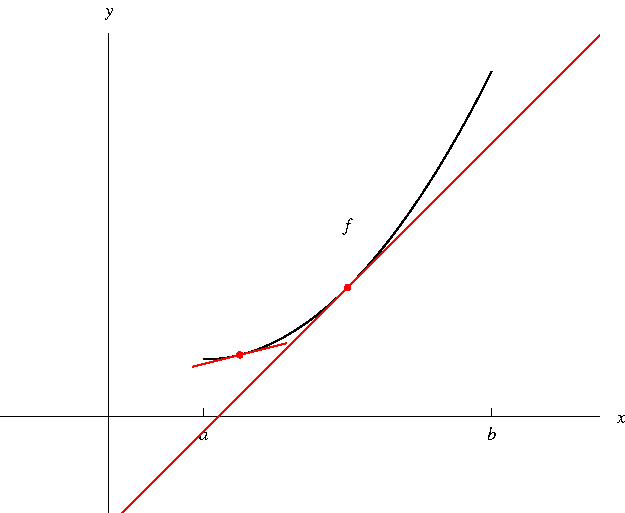
\includegraphics[height=3.5cm]{curve-sketching/pictures/04-03-concaveupc.pdf}%
}%
\only<handout:0| 5>{%
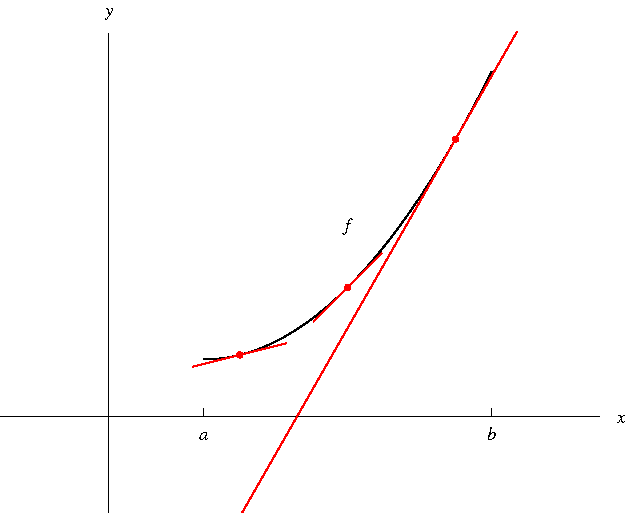
\includegraphics[height=3.5cm]{curve-sketching/pictures/04-03-concaveupd.pdf}%
}%
\only<6->{%
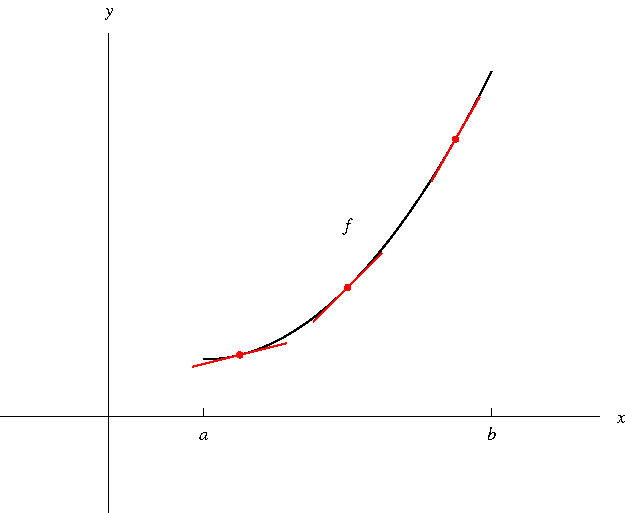
\includegraphics[height=3.5cm]{curve-sketching/pictures/04-03-concaveupe.pdf}%
}%

%\begin{center}
\ \ \ \ \ \ \ \ \ \uncover<6->{Concave up}
%\end{center}
\column{.5\textwidth}
\ \only<handout:0| -2>{%
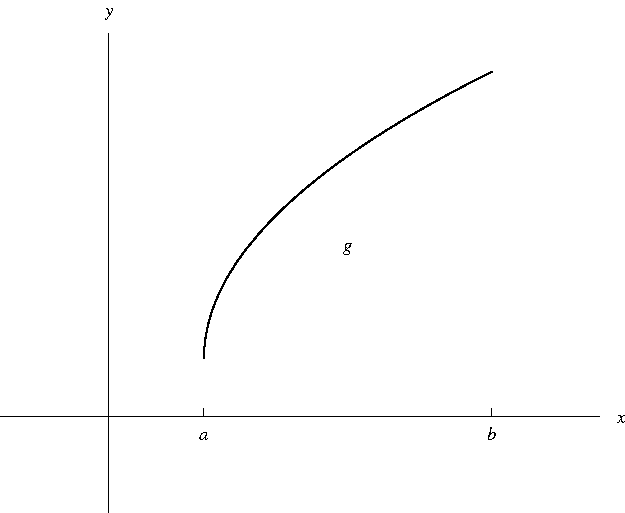
\includegraphics[height=3.5cm]{curve-sketching/pictures/04-03-concavedowna.pdf}%
}%
\only<handout:0| 3>{%
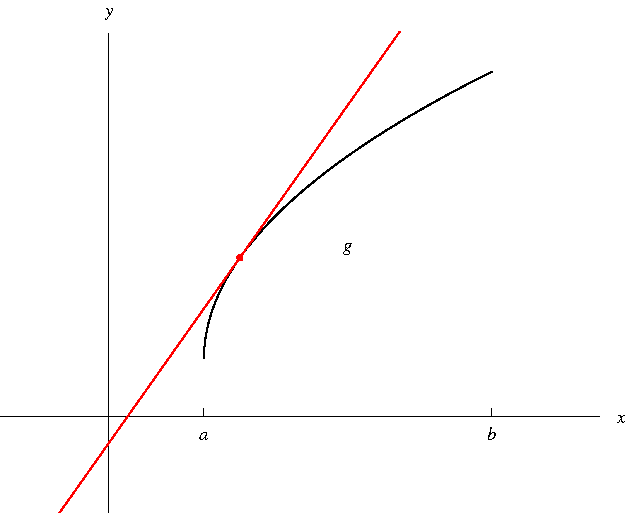
\includegraphics[height=3.5cm]{curve-sketching/pictures/04-03-concavedownb.pdf}%
}%
\only<handout:0| 4>{%
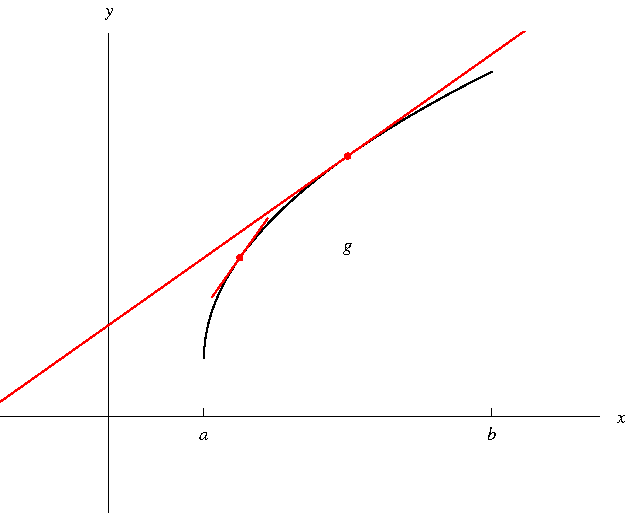
\includegraphics[height=3.5cm]{curve-sketching/pictures/04-03-concavedownc.pdf}%
}%
\only<handout:0| 5>{%
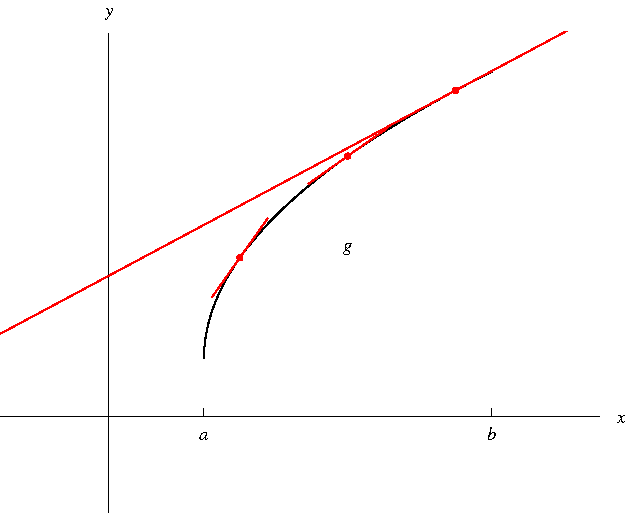
\includegraphics[height=3.5cm]{curve-sketching/pictures/04-03-concavedownd.pdf}%
}%
\only<6->{%
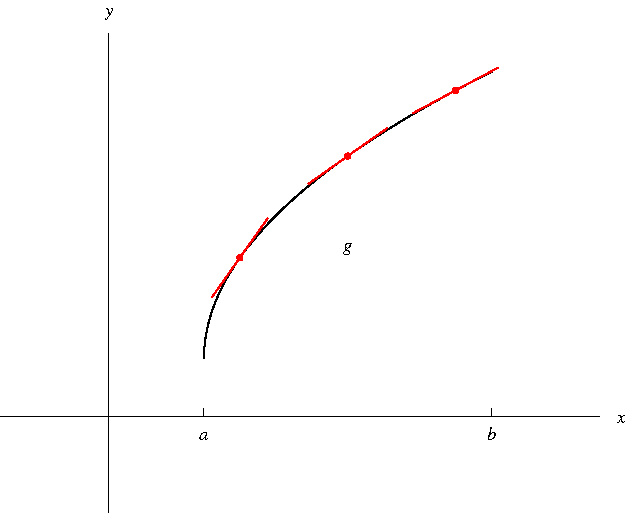
\includegraphics[height=3.5cm]{curve-sketching/pictures/04-03-concavedowne.pdf}%
}%

%\begin{center}
\ \ \ \ \ \ \ \ \ \uncover<6->{Concave down}
%\end{center}
\end{columns}
\uncover<2->{%
\begin{definition}[Concave Up/Concave Down]
Let $f$ be a differentiable function.  If the graph of $f$ lies above all of its tangents on an interval $I$, then it is called concave up on $I$.  If it lies below all of its tangents on $I$, it is called concave down on $I$.
\end{definition}
}%
\end{frame}
% end module concavity-def
